\documentclass{beamer}

\usepackage[english]{babel}
\usepackage[utf8x]{inputenc}
\usepackage[inline]{asymptote}
\usepackage{slide_helper}
\usepackage{caption}
\usepackage{subcaption}
\usepackage{comment}
\usepackage{tikz}
\usetikzlibrary{calc,patterns,decorations.pathmorphing,decorations.markings}

\title[MATH 2250 - Section 4.3]{Complex Characteristic Roots}

\begin{document}

\begin{frame}
  \titlepage
\end{frame}

\begin{frame}{Complex Characteristic Roots ($\Delta<0$)}
\begin{block}{Solution for Complex Characteristic Roots}
For $\Delta<0$, the characteristic roots of the DE

\vspace{-4mm}
\begin{equation*}
ay^{\prime\prime}+by^{\prime}+cy=0
\end{equation*}

\vspace{-5mm}
are
\begin{equation*}
\begin{aligned}
r_1&=\alpha+i\beta = -\dfrac{b}{2a}+i\dfrac{\sqrt{-(b^2-4ac)}}{2a}\\
r_2&=\alpha-i\beta = -\dfrac{b}{2a}-i\dfrac{\sqrt{-(b^2-4ac)}}{2a}
\end{aligned}
\end{equation*}\pause
The functions $e^{\alpha t}\cos[\beta t]$ and $e^{\alpha t}\sin[\beta t]$ are linearly independent solutions, and the general solution is given by
\begin{equation*}
y(t)=e^{\alpha t}\left(c_1\cos[\beta t]+c_2\sin[\beta t]\right)
\end{equation*}
where $c_1$ and $c_2$ are arbitrary constants determined by the initial conditions.\pause

The set $\left\{e^{\alpha t}\cos[\beta t],e^{\alpha t}\sin[\beta t]\right\}$ forms a basis for the solution space $\Sol$.
\end{block}
\end{frame}

\begin{frame}[fragile]{Complex Characteristic Roots ($\Delta<0$)}
\begin{example}
\begin{overprint}
\onslide<1-5>
Let us find the general solution of
\begin{equation*}
y^{\prime\prime}-4y^{\prime}+13y=0
\end{equation*}
\visible<2->{First, let us write the characteristic equation:
\begin{equation*}
0=r^2-4r+13
\end{equation*}}
\visible<3->{which has solutions $r=2\pm3i$. So $\alpha=2$ and $\beta=3$.}
\visible<4->{

Thus, the general solution is 
\begin{equation*}
y(t)=e^{2 t}\left(c_1\cos[3 t]+c_2\sin[3 t]\right)
\end{equation*}}
\visible<5->{The set $\left\{e^{2 t}\cos[3 t],e^{\alpha t}\sin[3 t]\right\}$ is a basis of the solution space $\Sol$,\linebreak and $\dim\Sol=2$.}
\onslide<6->
\begin{figure}
\centering
\begin{subfigure}[b]{0.4\textwidth}
\begin{asy}
import graph;
import fontsize;
defaultpen(fontsize(9pt));
size(150,150,IgnoreAspect);
ngraph=1000;
real min_x=-1, max_x=3;
real min_y=-300, max_y=300;

int pen_pos=-1;
pen[] pens={blue, red, heavycyan, heavymagenta, lightolive};
pens.cyclic=true;

pen next_color() {return pens[++pen_pos];}

real alpha=2;
real beta=3;
pair[] curves = {	( 4.0, 1.0), 
					( 2.0, 1.0), 
					(-2.0, 1.0),
					(-4.0, 1.0)};
					
for (pair k : curves)
{
	real A=k.x;
	real B=k.y;
	real c_1=A;
	real c_2=(B-A*alpha)/beta;
	real f(real t) {return exp(alpha*t)*(c_1*cos(beta*t)+c_2*sin(beta*t));}
	draw(graph(f,min_x, max_x),next_color()+0.75bp);
}
limits((min_x,min_y),(max_x,max_y),Crop);
xaxis("$t$",YEquals(0),min_x,max_x,Ticks(NoZero));
yaxis("$y$",XEquals(0),min_y,max_y,Ticks(NoZero));
\end{asy}
\caption{Time Series}
\end{subfigure}
\begin{subfigure}[b]{0.4\textwidth}
\begin{asy}
import graph;
import slopefield;
import fontsize;
defaultpen(fontsize(9pt));
size(150);
ngraph=1000;
real min_x=-600, max_x=600;
real min_y=-600, max_y=600;

pair start=(min_x,min_y);
pair end=(max_x,max_y);

real length(pair z) {return (z.x == 0) && (z.y == 0) ? 0.0001 : sqrt(z.x*z.x+z.y*z.y);}

// phase plot for ay''+by'+cy=0
real a=1;
real b=-4;
real c=13;
real F(pair z) {return (-b*z.y-c*z.x)/a;}
path vector(pair z) {return (0,0)--1/(2*length((z.y,F(z))))*(z.y, F(z));}

add(vectorfield(vector,start,end,arrow=EndArrow(SimpleHead)));

for(real gx=min_x+1; gx<=max_x-1; gx+=100)
	draw((gx,min_y)--(gx,max_y),dotted+darkgray);
    
for(real gy=min_y+1; gy<=max_y-1; gy+=100)
	draw((min_x,gy)--(max_x,gy),dotted+darkgray); 

// draw trajectories
int pen_pos=-1;
pen[] pens={blue, red, heavycyan, heavymagenta, lightolive};
pens.cyclic=true;
pen next_color() {return pens[++pen_pos];}

DefaultHead.size=new real(pen p=currentpen) {return 2.5mm;};

real alpha=2;
real beta=3;
real t_start=-1;
real t_end=3;

triple[] curves = {	( 4.0, 1.0, 0.2), 
					( 2.0, 1.0, 0.2), 
					(-2.0, 1.0, 0.2),
					(-4.0, 1.0, 0.2)};
			
for (triple k : curves)
{
	real A=k.x;
	real B=k.y;
	real c_1=A;
	real c_2=(B-A*alpha)/beta;
	real X(real t) {return exp(alpha*t)*(c_1*cos(beta*t)+c_2*sin(beta*t));}
	real Y(real t) {return exp(alpha*t)*(c_1*alpha*cos(beta*t) + c_2*alpha*sin(beta*t)-c_1*beta*sin(beta*t)+c_2*beta*cos(beta*t));}
	draw(graph(X,Y,t_start,t_end),next_color()+1.0bp,Arrow(Relative(k.z)));
}

limits(start,end,Crop);

xaxis("$y$",YEquals(min_y),min_x,max_x,LeftTicks());
xaxis(YEquals(max_y),min_x,max_x);
yaxis("$y^\prime$",XEquals(min_x),min_y,max_y,LeftTicks());
yaxis(XEquals(max_x),min_y,max_y);
\end{asy}
\caption{Phase Portrait}
\end{subfigure}
\end{figure}
\end{overprint}
\end{example}
\end{frame}

\begin{frame}[fragile]{Complex Characteristic Roots ($\Delta<0$)}
\begin{example}
\begin{overprint}
\onslide<1-5>
Let us find the general solution of
\begin{equation*}
y^{\prime\prime}+2y^{\prime}+4y=0
\end{equation*}
\visible<2->{First, let us write the characteristic equation:
\begin{equation*}
0=r^2+2r+4
\end{equation*}}
\visible<3->{which has solutions $r=-1\pm i\sqrt{3}$. So $\alpha=-1$ and $\beta=\sqrt{3}$.}
\visible<4->{

Thus, the general solution is 
\begin{equation*}
y(t)=e^{- t}\left(c_1\cos[\sqrt{3} t]+c_2\sin[\sqrt{3} t]\right)
\end{equation*}}
\visible<5->{The set $\left\{e^{- t}\cos[\sqrt{3} t],e^{-t}\sin[\sqrt{3} t]\right\}$ is a basis of the solution space $\Sol$,\linebreak and $\dim\Sol=2$.}
\onslide<6->
\begin{figure}
\centering
\begin{subfigure}[b]{0.4\textwidth}
\begin{asy}
import graph;
import fontsize;
defaultpen(fontsize(9pt));
size(150,0);
ngraph=1000;
real min_x=0, max_x=4;
real min_y=-2.5, max_y=2.5;

int pen_pos=-1;
pen[] pens={blue, red, heavycyan, heavymagenta, lightolive};
pens.cyclic=true;

pen next_color() {return pens[++pen_pos];}

real alpha=-1;
real beta=sqrt(3);
pair[] curves = {	( 0.0, -5.8), 
					( 0.0, -1.6), 
					( 0.0,  3.0),
					( 0.0,  5.0)};
					
for (pair k : curves)
{
	real A=k.x;
	real B=k.y;
	real c_1=A;
	real c_2=(B-A*alpha)/beta;
	real f(real t) {return exp(alpha*t)*(c_1*cos(beta*t)+c_2*sin(beta*t));}
	draw(graph(f,min_x, max_x),next_color()+0.75bp);
}
limits((min_x,min_y),(max_x,max_y),Crop);
xaxis("$t$",YEquals(0),min_x,max_x,Ticks(NoZero));
yaxis("$y$",XEquals(0),min_y,max_y,Ticks(NoZero));
\end{asy}
\caption{Time Series}
\end{subfigure}
\begin{subfigure}[b]{0.4\textwidth}
\begin{asy}
import graph;
import slopefield;
import fontsize;
defaultpen(fontsize(9pt));
size(150);
ngraph=1000;
real min_x=-12, max_x=12;
real min_y=-12, max_y=12;

pair start=(min_x,min_y);
pair end=(max_x,max_y);

real length(pair z) {return (z.x == 0) && (z.y == 0) ? 0.0001 : sqrt(z.x*z.x+z.y*z.y);}

// phase plot for ay''+by'+cy=0
real a=1;
real b=2;
real c=4;
real F(pair z) {return (-b*z.y-c*z.x)/a;}
path vector(pair z) {return (0,0)--1/(2*length((z.y,F(z))))*(z.y, F(z));}

add(vectorfield(vector,start,end,arrow=EndArrow(SimpleHead)));

for(real gx=min_x+1; gx<=max_x-1; gx+=2)
	draw((gx,min_y)--(gx,max_y),dotted+darkgray);
    
for(real gy=min_y+1; gy<=max_y-1; gy+=2)
	draw((min_x,gy)--(max_x,gy),dotted+darkgray); 

// draw trajectories
int pen_pos=-1;
pen[] pens={blue, red, heavycyan, heavymagenta, lightolive};
pens.cyclic=true;
pen next_color() {return pens[++pen_pos];}

DefaultHead.size=new real(pen p=currentpen) {return 2.5mm;};

real alpha=-1;
real beta=sqrt(3);
real t_start=-2;
real t_end=4;

triple[] curves = {	( 0.0, -5.8, 0.6), 
					( 0.0, -1.6, 0.25), 
					( 0.0,  3.0, 0.65),
					( 0.0,  5.0, 0.6)};
					
for (triple k : curves)
{
	real A=k.x;
	real B=k.y;
	real c_1=A;
	real c_2=(B-A*alpha)/beta;
	real X(real t) {return exp(alpha*t)*(c_1*cos(beta*t)+c_2*sin(beta*t));}
	real Y(real t) {return exp(alpha*t)*(c_1*alpha*cos(beta*t) + c_2*alpha*sin(beta*t)-c_1*beta*sin(beta*t)+c_2*beta*cos(beta*t));}
	draw(graph(X,Y,t_start,t_end),next_color()+1.0bp,Arrow(Relative(k.z)));
}

limits(start,end,Crop);

xaxis("$y$",YEquals(min_y),min_x,max_x,LeftTicks());
xaxis(YEquals(max_y),min_x,max_x);
yaxis("$y^\prime$",XEquals(min_x),min_y,max_y,LeftTicks());
yaxis(XEquals(max_x),min_y,max_y);
\end{asy}
\caption{Phase Portrait}
\end{subfigure}
\end{figure}
\end{overprint}
\end{example}
\end{frame}

\begin{frame}[fragile]{Complex Characteristic Roots ($\Delta<0$)}
\begin{example}
\begin{overprint}
\onslide<1-5>
Let us find the general solution of
\begin{equation*}
y^{\prime\prime}+y=0
\end{equation*}
\visible<2->{First, let us write the characteristic equation:
\begin{equation*}
0=r^2+1
\end{equation*}}
\visible<3->{which has solutions $r=\pm i$. So $\alpha=0$ and $\beta=1$.}
\visible<4->{

Thus, the general solution is 
\begin{equation*}
y(t)=c_1\cos[t]+c_2\sin[t]
\end{equation*}}
\visible<5->{The set $\left\{\cos[t],\sin[t]\right\}$ is a basis of the solution space $\Sol$,\linebreak and $\dim\Sol=2$.}
\onslide<6->
\begin{figure}
\centering
\begin{subfigure}[b]{0.4\textwidth}
\begin{asy}
import graph;
import fontsize;
defaultpen(fontsize(9pt));
size(150,0);
ngraph=1000;
real min_x=-3*pi, max_x=3*pi;
real min_y=-8, max_y=8;

int pen_pos=-1;
pen[] pens={blue, red, heavycyan, heavymagenta, lightolive};
pens.cyclic=true;

pen next_color() {return pens[++pen_pos];}

real alpha=0;
real beta=-1;
for (real i=1.0; i <= 5.0; i+=1.0)
{
	real A=i;
	real B=0;
	real c_1=A;
	real c_2=(B-A*alpha)/beta;
	real f(real t) {return exp(alpha*t)*(c_1*cos(beta*t)+c_2*sin(beta*t));}
	draw(graph(f,min_x, max_x),next_color()+0.75bp);
}
limits((min_x,min_y),(max_x,max_y),Crop);
xaxis("$t$",YEquals(0),min_x,max_x,Ticks(NoZero));
yaxis("$y$",XEquals(0),min_y,max_y,Ticks(NoZero));
\end{asy}
\caption{Time Series}
\end{subfigure}
\begin{subfigure}[b]{0.4\textwidth}
\begin{asy}
import graph;
import slopefield;
import fontsize;
defaultpen(fontsize(9pt));
size(150);
ngraph=1000;
real min_x=-6, max_x=6;
real min_y=-6, max_y=6;

int pen_pos=-1;
pen[] pens={blue, red, heavycyan, heavymagenta, lightolive};
pens.cyclic=true;

pen next_color() {return pens[++pen_pos];}

pair start=(min_x,min_y);
pair end=(max_x,max_y);

real length(pair z) {return (z.x == 0) && (z.y == 0) ? 0.0001 : sqrt(z.x*z.x+z.y*z.y);}

// phase plot for ay''+by'+cy=0
real a=1;
real b=0;
real c=1;
real F(pair z) {return (-b*z.y-c*z.x)/a;}
path vector(pair z) {return (0,0)--1/(2*length((z.y,F(z))))*(z.y, F(z));}

add(vectorfield(vector,start,end,arrow=EndArrow(SimpleHead)));

for(real gx=min_x+1; gx<=max_x-1; ++gx)
	draw((gx,min_y)--(gx,max_y),dotted+darkgray);
    
for(real gy=min_y+1; gy<=max_y-1; ++gy)
	draw((min_x,gy)--(max_x,gy),dotted+darkgray); 

// draw trajectories
DefaultHead.size=new real(pen p=currentpen) {return 2.5mm;};
real alpha=0;
real beta=1;
real t_start=0;
real t_end=2*pi;
for (real i=1.0; i <= 5.0; i+=1.0)
{
	real A=0;
	real B=i;
	real c_1=A;
	real c_2=(B-A*alpha)/beta;
	real X(real t) {return exp(alpha*t)*(c_1*cos(beta*t)+c_2*sin(beta*t));}
	real Y(real t) {return exp(alpha*t)*(c_1*alpha*cos(beta*t) + c_2*alpha*sin(beta*t)-c_1*beta*sin(beta*t)+c_2*beta*cos(beta*t));}
	draw(graph(X,Y,t_start,t_end),next_color()+1.0bp,MidArrow());
}

limits(start,end,Crop);

xaxis("$y$",YEquals(min_y),min_x,max_x,LeftTicks());
xaxis(YEquals(max_y),min_x,max_x);
yaxis("$y^\prime$",XEquals(min_x),min_y,max_y,LeftTicks());
yaxis(XEquals(max_x),min_y,max_y);
\end{asy}
\caption{Phase Portrait}
\end{subfigure}
\end{figure}
\end{overprint}
\end{example}
\end{frame}

\begin{frame}{Damped Mass-Spring Systems}
\begin{block}{Underdamped Mass-Spring System}
The motion of a mass-spring system is called \textbf{underdamped} when we have $\Delta=b^2-4mk<0$. Both characteristic roots are complex and the solutions are given by
\begin{equation*}
x(t)=e^{-\tfrac{b}{2m}}\left(c_1\cos[\omega_d t]+c_2\sin[\omega_d t]\right)
,\quad
\omega_d=\dfrac{\sqrt{4mk-b^2}}{2m}
\end{equation*}
\end{block}
\end{frame}

\begin{frame}{Damped Mass-Spring Systems}
\begin{block}{Alternate Solution to the Underdamped Unforced Oscillator}
\begin{equation*}
x(t)=A(t)\cos[\omega_d t - \delta]
,\quad
\omega_d=\dfrac{\sqrt{4mk-b^2}}{2m}
\end{equation*}
Where $A$ and $\delta$ are determined by initial conditions, the following hold:
\begin{dynitemize}[<+- | alert@+>]
\item\textbf{Time-varying amplitude} $A(t)=Ae^{-\tfrac{b}{2m}}$
\item\textbf{Phase angle} $\delta$
\item\textbf{Phase shift} $\varphi=\dfrac{\delta}{\omega_d}$
\item\textbf{Circular quasi-frequency} $\omega_d$
\item\textbf{Natural quasi-frequency} $f_d=\dfrac{\omega_d}{2\pi}$
\item\textbf{Quasi-period} $T_d=\dfrac{1}{f_d}=\dfrac{2pi}{\omega_d}$
\item\textbf{Time constant} $\tau=\dfrac{2m}{b}$
\end{dynitemize}
\end{block}
\end{frame}

\begin{frame}[fragile]{Damped Mass-Spring Systems}
\begin{block}{Alternate Solution to the Underdamped Unforced Oscillator}
\begin{center}
\begin{asy}
import graph;
import fontsize;
defaultpen(fontsize(9pt));
size(400, 180);
ngraph=1000;
real min_x=-2, max_x=20;
real min_y=-6, max_y=6;

pair start=(min_x, min_y);
pair end=(max_x, max_y);

real m=5;
real b=0.75;
real k=2;
real A=5;
//real delta=0;

real omega=sqrt(4*m*k-b*b)/(2*m);
real delta=omega+0.5;

real quasiperiod=2*pi/omega;
real start_y=A*cos(delta);
real xtick(int i) { return (delta+(i-1)*pi)/omega-0.2;}

real A(real t) {return A*exp((-1*(b/(2*m)))*t);}
real negA(real t) {return -1*A(t);}
real x(real t) {return A(t)*cos(omega*t-delta);}

pen line_pen=black+0.75bp;
pen amp_pen=dashed+deepgreen+0.5bp;
pen mark_pen=dashed+deepred+0.5bp;
pen arrow_pen=deepred+0.5bp;
pen text_pen=blue+0.5bp;

draw(graph(A, 0, max_x),amp_pen);
label("$Ae^{-\tfrac{b}{2m}}$", (xtick(4), A(xtick(4))+0.75), text_pen, UnFill);

draw(graph(negA,0, max_x), amp_pen);
label("$-Ae^{-\tfrac{b}{2m}}$", (xtick(1)+1, negA(xtick(4))-3.3), text_pen, NoFill);

draw(graph(x, 0, max_x), line_pen);

draw((min_x, start_y)--(0, start_y), mark_pen);
draw((min_x/2, start_y)--(min_x/2, 0), arrow_pen, Arrows);
label("$A\cos\delta$", (min_x/2, start_y/2), text_pen, UnFill);

real qp_height=max_y*0.9;
draw((xtick(1), x(xtick(1)))--(xtick(1), max_y), mark_pen);
draw((xtick(3), x(xtick(3)))--(xtick(3), max_y), mark_pen);
draw((xtick(1), qp_height)--(xtick(3), qp_height), arrow_pen, Arrows);
label("Quasi-period $\dfrac{2\pi}{\omega_d}$", (xtick(2), qp_height), text_pen, UnFill);

limits(start, end, Crop);

xaxis("$t$", YEquals(0), min_x, max_x, NoTicks());
yaxis("$x$", XEquals(0), min_y, max_y, NoTicks());

real tick_height=0.2;
for (int i = 1; i <= 4; ++i)
{
	draw((xtick(i), tick_height)--(xtick(i), 0), mark_pen);
	draw((xtick(i), -1*tick_height)--(xtick(i), 0), mark_pen);
}	

label("$\delta/\omega_d$", (xtick(1), -0.75), text_pen, UnFill);
label("$(\delta+\pi)/\omega_d$", (xtick(2), +0.75), text_pen, UnFill);
label("$(\delta+2\pi)/\omega_d$", (xtick(3), -0.75), text_pen, UnFill);
label("$(\delta+3\pi)/\omega_d$", (xtick(4), +0.75), text_pen, UnFill);
\end{asy}
\end{center}
\end{block}
\end{frame}

\begin{frame}[fragile]{Underdamped Mass-Spring System}
\begin{example}
\begin{overprint}
\onslide<1-4>
Consider the Mass-Spring IVP where
\begin{equation*}
\ndot{x}{2}+\ndot{x}{1}+x=0
,\quad
x(0)=1
,\quad
\ndot{x}{1}(0)=0
\end{equation*}

\visible<2->{which has characteristic equation
\begin{equation*}
r^2+r+1=0
\end{equation*}}

\visible<3->{and characteristic solutions
\begin{equation*}
r=-\dfrac{1}{2}\pm i\dfrac{\sqrt{3}}{2}
\end{equation*}}

\visible<4->{Which means $\alpha=-\dfrac{1}{2}$ and $\beta=\dfrac{\sqrt{3}}{2}$.}
\onslide<5-7>
The general solution is
\begin{equation*}
x(t)=
e^{-\tfrac{t}{2}}
\left(
	 c_1\cos[\dfrac{\sqrt{3}}{2}t]
	+c_2\sin[\dfrac{\sqrt{3}}{2}t]
\right)
\end{equation*}

\visible<6->{We can then calculate
\begin{equation*}
\ndot{x}{1}(t)=
e^{-\tfrac{t}{2}}
\left(
	\left(
		-\dfrac{c_1}{2}
		+\dfrac{c_2\sqrt{3}}{2}
	\right)
	\cos[\dfrac{t\sqrt{3}}{2}]
	-
	\left(
		 \dfrac{c_2}{2}
		+\dfrac{c_2\sqrt{3}}{2}
	\right)
	\sin[\dfrac{t\sqrt{3}}{2}]
\right)
\end{equation*}}

\visible<7->{If we substitute in the initial conditions $x(0)=1$ and $\ndot{x}{1}(0)=0$,\\ we find that $c_1=1$ and $c_2=\dfrac{1}{\sqrt{3}}$.}
\onslide<8-9>
Thus, the solution to the IVP is 
\begin{equation*}
x(t)=
e^{-\tfrac{t}{2}}
\left(
	 \cos[\dfrac{\sqrt{3}}{2}t]
	+\dfrac{1}{\sqrt{3}}\sin[\dfrac{\sqrt{3}}{2}t]
\right)
\end{equation*}

\visible<9->{
In alternate polar form
\begin{equation*}
x(t)=
\dfrac{2}{\sqrt{3}}e^{-\tfrac{t}{2}}
\cos[\dfrac{\sqrt{3}}{2}t - \dfrac{\pi}{6}]
\end{equation*}

Where
\begin{equation*}
A=\sqrt{1^2+{\left(\dfrac{1}{\sqrt{3}}\right)}^2}=\dfrac{2}{\sqrt{3}}
\quad\text{and}\quad
\delta=\tan^{-1}\left(\dfrac{\tfrac{1}{\sqrt{3}}}{1}\right)=\dfrac{\pi}{6}
\end{equation*}}
\onslide<10-15>
\begin{equation*}
x(t)=
\dfrac{2}{\sqrt{3}}e^{-\tfrac{t}{2}}
\cos[\dfrac{\sqrt{3}}{2}t - \dfrac{\pi}{6}]
\end{equation*}

Has the following properties:
\begin{dynitemize}
\item<11- | alert@11> time-varying amplitude $A(t)=\dfrac{2}{\sqrt{3}}e^{-\tfrac{t}{2}}$.
\item<12- | alert@12> circular quasi-frequency $\omega_d=\dfrac{\sqrt{3}}{2}$
\item<13- | alert@13> natural quasi-frequency $f_d=\dfrac{\omega_d}{2\pi}=\dfrac{\sqrt{3}}{4\pi}$ hertz
\item<14- | alert@14> quasi-period $T_d=\dfrac{2\pi}{\omega_d}=\dfrac{4\pi}{\sqrt{3}}$ seconds
\item<15- | alert@15> phase-shift $\varphi=\dfrac{\delta}{\omega_d}=\dfrac{\pi}{3\sqrt{3}}$ rad per second
\end{dynitemize}
\onslide<16->
\begin{figure}
\centering
\begin{subfigure}[b]{0.4\textwidth}
\begin{asy}
import graph;
import fontsize;
defaultpen(fontsize(9pt));
size(120);
ngraph=1000;
real min_x=-6, max_x=6;
real min_y=-6.5, max_y=6.5;

int pen_pos=-1;
pen[] pens={blue, red, heavycyan, heavymagenta, lightolive};
pens.cyclic=true;

pen next_color() {return pens[++pen_pos];}

real alpha=-1/2;
real beta=sqrt(3)/2;

real A=1;
real B=0;
real c_1=A;
real c_2=(B-A*alpha)/beta;
real f(real t) {return exp(alpha*t)*(c_1*cos(beta*t)+c_2*sin(beta*t));}
draw(graph(f,min_x, max_x),next_color()+0.75bp);

limits((min_x,min_y),(max_x,max_y),Crop);
xaxis("$t$",YEquals(0),min_x,max_x,Ticks(NoZero));
yaxis("$x$",XEquals(0),min_y,max_y,Ticks(NoZero));
\end{asy}
\caption{Time Series}
\end{subfigure}
\begin{subfigure}[b]{0.4\textwidth}
\begin{asy}
import graph;
import slopefield;
import fontsize;
defaultpen(fontsize(9pt));
size(120);
ngraph=1000;
real min_x=-7, max_x=7;
real min_y=-7, max_y=7;

int pen_pos=-1;
pen[] pens={blue, red, heavycyan, heavymagenta, lightolive};
pens.cyclic=true;

pen next_color() {return pens[++pen_pos];}

pair start=(min_x,min_y);
pair end=(max_x,max_y);

real length(pair z) {return (z.x == 0) && (z.y == 0) ? 0.0001 : sqrt(z.x*z.x+z.y*z.y);}

// phase plot for ay''+by'+cy=0
real a=1;
real b=1;
real c=1;
real F(pair z) {return (-b*z.y-c*z.x)/a;}
path vector(pair z) {return (0,0)--1/(2*length((z.y,F(z))))*(z.y, F(z));}

add(vectorfield(vector,start,end,arrow=EndArrow(SimpleHead)));

for(real gx=min_x+1; gx<=max_x-1; ++gx)
	draw((gx,min_y)--(gx,max_y),dotted+darkgray);
    
for(real gy=min_y+1; gy<=max_y-1; ++gy)
	draw((min_x,gy)--(max_x,gy),dotted+darkgray); 

// draw trajectories
DefaultHead.size=new real(pen p=currentpen) {return 2.5mm;};
real alpha=-1/2;
real beta=sqrt(3)/2;
real t_start=-1.5*pi;
real t_end=2*pi;

real A=1;
real B=0;
real c_1=A;
real c_2=(B-A*alpha)/beta;
real X(real t) {return exp(alpha*t)*(c_1*cos(beta*t)+c_2*sin(beta*t));}
real Y(real t) {return exp(alpha*t)*(c_1*alpha*cos(beta*t) + c_2*alpha*sin(beta*t)-c_1*beta*sin(beta*t)+c_2*beta*cos(beta*t));}
draw(graph(X,Y,t_start,t_end),next_color()+1.0bp,MidArrow());

limits(start,end,Crop);

xaxis("$x$",YEquals(min_y),min_x,max_x,LeftTicks());
xaxis(YEquals(max_y),min_x,max_x);
yaxis("$x^\prime$",XEquals(min_x),min_y,max_y,LeftTicks());
yaxis(XEquals(max_x),min_y,max_y);
\end{asy}
\caption{Phase Portrait}
\end{subfigure}
\end{figure}
\end{overprint}
\end{example}
\end{frame}

\begin{frame}{The Guitar String: A Qualitative Analysis}
\begin{block}{}
The vibration of a guitar string can be described as a damped oscillator.
\begin{columns}
\begin{column}{0.4\textwidth}
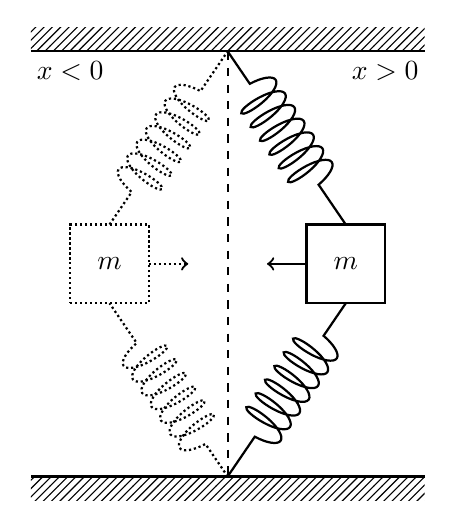
\begin{tikzpicture}[every node/.style={outer sep=0pt,thick}]
\tikzstyle{spring}=[thick,decorate,decoration={coil,pre length=0.5cm,post length=0.5cm,segment length=6, amplitude=3mm, aspect=0.3}]
\tikzstyle{damper}=[thick,decoration={markings,  
  mark connection node=dmp,
  mark=at position 0.5 with 
  {
    \node (dmp) [thick,inner sep=0pt,transform shape,rotate=-90,minimum width=15pt,minimum height=3pt,draw=none] {};
    \draw [thick] ($(dmp.north east)+(2pt,0)$) -- (dmp.south east) -- (dmp.south west) -- ($(dmp.north west)+(2pt,0)$);
    \draw [thick] ($(dmp.north)+(0,-5pt)$) -- ($(dmp.north)+(0,5pt)$);
  }
}, decorate]
\tikzstyle{ground}=[fill,pattern=north east lines,draw=none,minimum width=0.75cm,minimum height=0.3cm]

%\node (Center) {};
\coordinate (Center) (0,0);
\node (ceiling) [draw, ground,anchor=north,yshift=+3cm,minimum width=5cm] at (Center.north) {};
\draw [thick] (ceiling.south east) -- (ceiling.south west);

\node (ground) [draw, ground,anchor=south,yshift=-3cm,minimum width=5cm] at (Center.south) {};
\draw [thick] (ground.north east) -- (ground.north west);

\draw [dashed, thick] ($(ceiling.south west)!0.5!(ceiling.south east)$) -- ($(ground.north west)!0.5!(ground.north east)$);

\node [yshift=-0.25cm, xshift=-0.5cm] at (ceiling.south east) {$x>0$};
\node [yshift=-0.25cm, xshift=0.5cm] at (ceiling.south west) {$x<0$};

\node (M1) [draw, minimum width=1cm, minimum height=1cm, xshift=+1.5cm] at (Center.east) {$m$};

\draw [spring] ($(ceiling.south west)!0.5!(ceiling.south east)$) -- ($(M1.north west)!0.5!(M1.north east)$);
\draw [spring] ($(M1.south west)!0.5!(M1.south east)$) -- ($(ground.north west)!0.5!(ground.north east)$);

\draw [thick, ->] ($(M1.north west)!0.5!(M1.south west)$) -* (0.5,0);

\node (M2) [draw, densely dotted, minimum width=1cm, minimum height=1cm, xshift=-1.5cm] at (Center.east) {$m$};

\draw [densely dotted, spring] ($(M2.north west)!0.5!(M2.north east)$) -- ($(ceiling.south west)!0.5!(ceiling.south east)$);
\draw [densely dotted, spring] ($(ground.north west)!0.5!(ground.north east)$) -- ($(M2.south west)!0.5!(M2.south east)$);

\draw [densely dotted, thick, ->] ($(M2.north east)!0.5!(M2.south east)$) -* (-0.5,0);
\end{tikzpicture}
\end{column}
\begin{column}{0.55\textwidth}
\pause
The motion of this spring is given by
\begin{equation*}
\ndot{x}{2}+\omega_0^2 x=0
\end{equation*}
where $\omega_0$ is the circular frequency at which the string vibrates. (In music, the frequency $f_0=\tfrac{\omega_o}{2\pi}$ is often used. A middle C has 512 vibrations per second.)\pause

Because there is no damping in this model, the sound will last forever.\pause

When a guitar string is plucked, it has the $x(0)=x_0$ and $\ndot{x}{1}(0)=0$ for initial conditions.
\end{column}
\end{columns}
\end{block}\pause

\begin{block}{}
Let use next consider a guitar string with damping.
\end{block}
\end{frame}

\begin{frame}[fragile]{The Guitar String: A Qualitative Analysis}
\begin{example}
\begin{overprint}
\onslide<1-5>
Consider the underdamped guitar string
\begin{equation*}
\ndot{x}{2}+2\ndot{x}{1}+26x=0
\end{equation*}
\visible<2->{First, let us write the characteristic equation:
\begin{equation*}
0=r^2+2r+26
\end{equation*}}
\visible<3->{which has solutions $r=-1\pm5i$. So $\alpha=-1$ and $\beta=5$.}
\visible<4->{

Thus, the general solution is 
\begin{equation*}
x(t)=e^{- t}\left(c_1\cos[5 t]+c_2\sin[5 t]\right)
\end{equation*}}
\visible<5->{

If we pluck the string, which means $x(0)=5$ and $\ndot{x}{1}(0)=0$, we find that $c_1=5$ and $c_2=1$.}
\onslide<6->
\begin{figure}
\centering
\begin{subfigure}[b]{0.4\textwidth}
\begin{asy}
import graph;
import fontsize;
defaultpen(fontsize(9pt));
size(0,150);
ngraph=1000;
real min_x=-1, max_x=8;
real min_y=-4, max_y=6;

int pen_pos=-1;
pen[] pens={blue, red, heavycyan, heavymagenta, lightolive};
pens.cyclic=true;

pen next_color() {return pens[++pen_pos];}

real alpha=-1;
real beta=5;

real A=5;
real B=0;
real c_1=A;
real c_2=(B-A*alpha)/beta;
real f(real t) {return exp(alpha*t)*(c_1*cos(beta*t)+c_2*sin(beta*t));}
draw(graph(f,0, max_x),next_color()+0.75bp);

limits((min_x,min_y),(max_x,max_y),Crop);
xaxis("$t$",YEquals(0),min_x,max_x,Ticks(NoZero));
yaxis("$x$",XEquals(0),min_y,max_y,Ticks(NoZero));
\end{asy}
\caption{Time Series}
\end{subfigure}
\begin{subfigure}[b]{0.4\textwidth}
\begin{asy}
import graph;
import slopefield;
import fontsize;
defaultpen(fontsize(9pt));
size(0,150);
ngraph=1000;
real min_x=-11, max_x=11;
real min_y=-11, max_y=11;

int pen_pos=-1;
pen[] pens={blue, red, heavycyan, heavymagenta, lightolive};
pens.cyclic=true;

pen next_color() {return pens[++pen_pos];}

pair start=(min_x,min_y);
pair end=(max_x,max_y);

real length(pair z) {return (z.x == 0) && (z.y == 0) ? 0.0001 : sqrt(z.x*z.x+z.y*z.y);}

// phase plot for ay''+by'+cy=0
real a=1;
real b=2;
real c=26;
real F(pair z) {return (-b*z.y-c*z.x)/a;}
path vector(pair z) {return (0,0)--1/(2*length((z.y,F(z))))*(z.y, F(z));}

add(vectorfield(vector,start,end,arrow=EndArrow(SimpleHead)));

for(real gx=min_x+1; gx<=max_x-1; ++gx)
	draw((gx,min_y)--(gx,max_y),dotted+darkgray);
    
for(real gy=min_y+1; gy<=max_y-1; ++gy)
	draw((min_x,gy)--(max_x,gy),dotted+darkgray); 

// draw trajectories
DefaultHead.size=new real(pen p=currentpen) {return 2.5mm;};
real alpha=-1;
real beta=5;
real t_start=0.4;
real t_end=10;

real A=5;
real B=0;
real c_1=A;
real c_2=(B-A*alpha)/beta;
real X(real t) {return exp(alpha*t)*(c_1*cos(beta*t)+c_2*sin(beta*t));}
real Y(real t) {return exp(alpha*t)*(c_1*alpha*cos(beta*t) + c_2*alpha*sin(beta*t)-c_1*beta*sin(beta*t)+c_2*beta*cos(beta*t));}
draw(graph(X,Y,t_start,t_end),next_color()+1.0bp,MidArrow());

limits(start,end,Crop);

xaxis("$x$",YEquals(min_y),min_x,max_x,LeftTicks());
xaxis(YEquals(max_y),min_x,max_x);
yaxis("$x^\prime$",XEquals(min_x),min_y,max_y,LeftTicks());
yaxis(XEquals(max_x),min_y,max_y);
\end{asy}
\caption{Phase Portrait}
\end{subfigure}
\end{figure}
\end{overprint}
\end{example}
\end{frame}

\begin{frame}{Real and Complex Characteristic Roots}
\begin{block}{Solutions to the Second-Order Linear DE with Constant Coefficients}
The differential equation

\vspace{-4mm}
\begin{equation*}
ay^{\prime\prime}+by^{\prime}+cy=0
\end{equation*}

\vspace{-3mm}
has the characteristic equation

\vspace{-4mm}
\begin{equation*}
ar^2+br+c=0
\end{equation*}

\vspace{-3mm}
The quadratic formula gives rise to three different general solutions, depending on the discriminant $\Delta=b^2-4ac$.

\vspace{-4mm}
\begin{center}
\def\arraystretch{1.8}%
\begin{tabular}{ccc}
& Characteristic Roots & General Solution \\
$\Delta>0$ & $r_1,r_2=\dfrac{-b\pm\sqrt{b^2-4ac}}{2a}$ & $y=c_1e^{r_1 t}+c_2e^{r_2 t}$\\
$\Delta=0$ & $r=-\dfrac{b}{2a}$ & $y=c_1e^{rt}+c_2te^{rt}$\\
$\Delta<0$ & $r_1,r_2=\alpha\pm\beta$ & $y=e^{\alpha t}\left(c_1\cos[\beta t]+c_2\sin[\beta t]\right)$ \\
&$\alpha=-\dfrac{b}{2a}$, $\beta=\dfrac{\sqrt{4ac-b^2}}{2a}$ &\\
\end{tabular}
\end{center}
\end{block}
\end{frame}

\begin{frame}{Extensions to Higher-Order DE}
\begin{example}
Consider the fourth-order DE

\vspace{-1mm}
\begin{equation*}
\dfrac{d^4 y}{dy^4}-16y=0
\end{equation*}\pause
It's characteristic equation is

\vspace{-1mm}
\begin{equation*}
\begin{aligned}
0=r^4-16\pause
=(r^2-4)(r^2+4)\pause
=(r+2)(r-2)(r^2+4)
\end{aligned}
\end{equation*}\pause

\vspace{-3mm}
Which has the characteristic solutions
\begin{equation*}
r_1 = 2  , \quad r_2  = -2 , \quad r_3 = 2i , \quad r_4  = -2i
\end{equation*}\pause

\vspace{-3mm}
Thus, $\{e^{2t},e^{-2t},\cos[2t],\sin[2t]\}$ form a basis of $\Sol$ and the general solution is
\begin{equation*}
y=c_1e^{2t}+c_2e^{-2t}+c_3\cos[2t]+c_4\sin[2t]
\end{equation*}
\end{example}
\end{frame}

\begin{frame}{Extensions to Higher-Order DE}
\begin{example}
Consider the third-order DE

\vspace{-1mm}
\begin{equation*}
y^{\prime\prime\prime}+y^{\prime\prime}-5y^{\prime}+3y=0
\end{equation*}\pause
It's characteristic equation is

\vspace{-1mm}
\begin{equation*}
\begin{aligned}
0=r^3+r^2-5r+3\pause
=(r-1)(r^2+2r-3)\pause
={(r-1)}^2(r+3)
\end{aligned}
\end{equation*}\pause

\vspace{-3mm}
Which has the characteristic solutions
\begin{equation*}
r_1=1, \quad r_2=1, \quad r_3=-3
\end{equation*}\pause

\vspace{-3mm}
Thus, $\{e^{t},te^{t},e^{-3t}\}$ form a basis of $\Sol$ and the general solution is
\begin{equation*}
y=c_1e^{t}+c_2te^{t}+c_3e^{-3t}
\end{equation*}
\end{example}
\end{frame}

\begin{frame}{Extensions to Higher-Order DE}
\begin{example}
Consider the fifth-order DE

\vspace{-1mm}
\begin{equation*}
\dfrac{d^5y}{dt^5}
+3\dfrac{d^4y}{dt^4}
+3\dfrac{d^3y}{dt^3}
+\dfrac{d^2y}{dt^2}
=0
\end{equation*}\pause
It's characteristic equation is

\vspace{-1mm}
\begin{equation*}
\begin{aligned}
0=r^5+3r^4+3r^3+r^2\pause
={(r+1)}^3r^2
\end{aligned}
\end{equation*}\pause

\vspace{-3mm}
Which has the characteristic solutions
\begin{equation*}
r_1=-1,\quad
r_2=-1,\quad
r_3=-1,\quad
r_4=0,\quad
r_5=0
\end{equation*}\pause

\vspace{-3mm}
Thus, $\{e^{-t},te^{-t},t^2e^{-t},1,t\}$ form a basis of $\Sol$ and the general solution is
\begin{equation*}
y=\underset{\text{\tiny for triple root}}{(c_1+c_2t+c_3t^2)}e^{-t}
 +\underset{\text{\tiny for double root}}{(c_4+c_5t)}
\end{equation*}
\end{example}
\end{frame}

\begin{frame}{Extensions to Higher-Order DE}
\begin{example}
Consider the fourth-order DE

\vspace{-1mm}
\begin{equation*}
\dfrac{d^4y}{dt^4}
+8\dfrac{d^2y}{dt^2}
+16y
=0
\end{equation*}\pause
It's characteristic equation is

\vspace{-1mm}
\begin{equation*}
\begin{aligned}
0=r^4+8r^2+16\pause
={(r^2+4)}^2
\end{aligned}
\end{equation*}\pause

\vspace{-3mm}
Which has the characteristic solutions
\begin{equation*}
r_1=2i,\quad
r_2=2i,\quad
r_3=-2i,\quad
r_4=-2i
\end{equation*}\pause

\vspace{-3mm}
Thus, $\{\cos[2t],t\cos[2t],\sin[2t],t\sin[2t]\}$ form a basis of $\Sol$ and the general solution is

\vspace{-4mm}
\begin{equation*}
y=\underset{\text{\tiny for double root}}{(c_1+c_2t)}\cos[2t]
 +\underset{\text{\tiny for double root}}{(c_3+c_4t)}\sin[2t]
\end{equation*}
\end{example}
\end{frame}
\end{document}